\usetikzlibrary{calc}



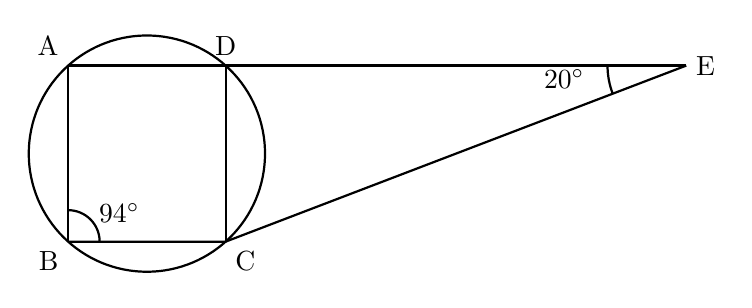
\begin{tikzpicture}[scale=1]

    % Define the center of the circle
    \coordinate (O) at (0,0);

    % Define the coordinates for the points on the circle
    % Adjusted B so that AB and CD are exactly parallel and equal (both vertical)
    \coordinate (A) at (-1, 1.118);
    \coordinate (B) at (-1, -1.118);
    \coordinate (C) at (1, -1.118);
    \coordinate (D) at (1, 1.118);

    % Define the external intersection point E
    \coordinate (E) at (6.85, 1.118);

    % Draw the circle
    \draw[thick] (O) circle (1.5);

    % Draw the lines forming the shape
    % Line from A through D extending to E
    \draw[thick] (A) -- (D) -- (E);
    
    % Line from B through C extending to E
    % Note: Making AB and CD parallel and equal forces ABCD to be a rectangle. 
    % For the lines to still intersect at E, the line will have a bend at C.
    \draw[thick] (B) -- (C) -- (E);
    
    % Vertical and side segments of the inscribed quadrilateral
    \draw[thick] (A) -- (B);
    \draw[thick] (D) -- (C);

    % Draw the angle arc at B
    % Since AB is now perfectly vertical and BC is perfectly horizontal, the angle is 90 degrees geometrically
    \draw[thick] (B) ++(0:0.4) arc (0:90:0.4);
    
    % Place the 94 degree label
    \node at (-0.35, -0.75) {$94^{\circ}$};

    % Draw the angle arc at E (20 degrees)
    % The line ED is horizontal (180 degrees), and EC is at approx 200.9 degrees
    \draw[thick] (E) ++(180:1.0) arc (180:200.9:1.0);
    
    % Place the 20 degree label
    \node at (5.3, 0.95) {$20^{\circ}$};

    % Add labels for all the vertices
    \node[above left] at (A) {A};
    \node[below left] at (B) {B};
    \node[below right] at (C) {C};
    \node[above] at (D) {D};
    \node[right] at (E) {E};

\end{tikzpicture}